\chapter{Platforma od strony użytkowej}
\label{chapter:interfaces}

W ramach platformy wyróżnia się dwa podstawowe interfejsy: prowadzącego i studenta.
Dla pierwszego z nich wyróżnia się dwa widoki: zarządzania projektami i podglądu postępów studentów.

\section{Interfejs prowadzącego}

\subsection{Zarządzanie projektami}

Na rysunku \ref{fig:lecturer-interface-management} został przedstawiony widok zarządzania projektami.
W ramach interfejsu udostępnione jest tworzenie i edytowanie projektów, w tym wyznaczanie etapów i dodawanie do nich przypadków testowych.
Definiowanie projektu przebiega następująco:
\begin {itemize}
    \item Prowadzący tworzy nowy projekt.
    \item Prowadzący tworzy etapy w ramach danego projektu.
    \item Prowadzący tworzy przypadki testowe dla etapów.
    \item Prowadzący tworzy procesy integracji w ramach danego projektu.
    \item Prowadzący tworzy grupy projektowe.
\end {itemize}

\begin{figure}[h]
    \centering
    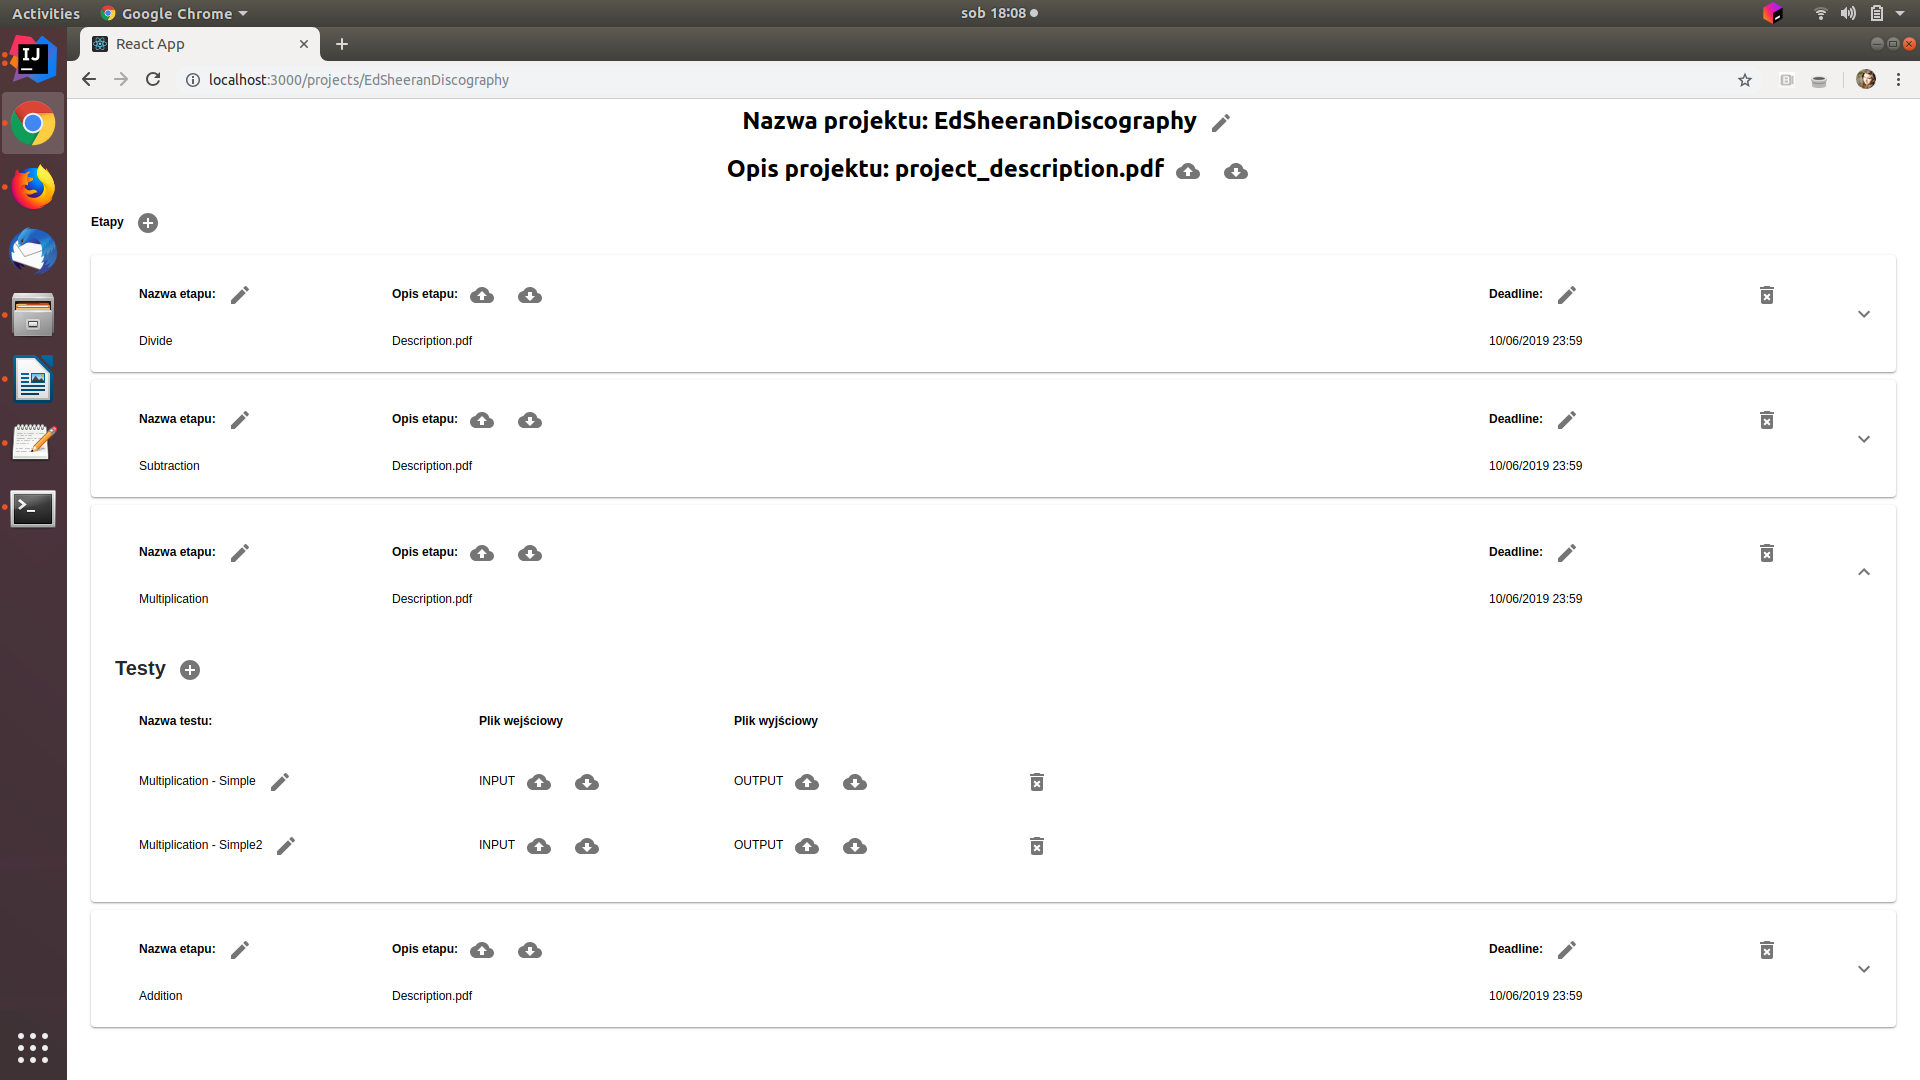
\includegraphics[width = 13cm]{chapter04/lecturer_interface_management.png}
    \caption{Interfejs prowadzącego - zarządzanie projektami (źródło własne).}
    \label{fig:lecturer-interface-management}
\end{figure}

Nowy projekt definiowany jest przez następujące dane:
\begin {itemize}
    \item Nazwę projektu, która jest jednoznaczna z nazwą katalogu na dysku, w którym przechowywane będą pliki z danymi dotyczącymi projektu.
    Nazwa jest parametrem będącym ciągiem znaków (String).
    \item Plik z opisem projektu o dowolnym formacie.
    \item Plik Dockerfile definiujący środowisko uruchomieniowe programów.
\end {itemize}

Lista dostępnych projektów jest posortowana alfabetycznie po ich nazwie.
Dla wszystkich parametrów będących plikami interfejs umożliwia dodanie ich poprzez wskazanie, w oknie dialogowym, ścieżki na dysku użytkownika, pod którą znajduje się plik.

Nowy etap definiowany jest przez następujące dane:
\begin {itemize}
    \item Nazwę etapu, która jest jednoznaczna z nazwą katalogu na dysku, w którym przechowywane będą pliki z danymi dotyczącymi etapu.
    Nazwa jest parametrem będącym ciągiem znaków (String).
    \item Plik z opisem etapu o dowolnym formacie.
    \item Metadane dotyczące etapu, takie jak:
    \begin {itemize}
        \item Data rozpoczęcia etapu.
        Data rozpoczęcia jest rozumiana jako data, od której studenci mają możliwość rozpoczęcia prac nad etapem (dostęp do opisu etapu, możliwość zaimportowania i uruchomienia swoich programów),
        \item Data zakończenia etapu.
        Data zakończenia jest rozumiana jako data, do której studenci mają możliwość zaimportowania i uruchomienia swoich programów.
        Po przekroczeniu tej daty zmian programów i ponownych uruchomień może dokonywać tylko prowadzący,
        \item Punktacja za wskazany etap, podawana w postaci liczby całkowitej.
        Na podstawie punktacji poszczególnych etapów zliczana jest automatycznie ocena końcowa dla projektu.
    \end{itemize}
\end {itemize}

Etapy, które nie mają zdefiniowanej daty rozpoczęcia nie są widoczne dla studentów.
Interfejs umożliwia wskazanie daty poprzez wybór jej w oknie dialogowym z kalendarzem.

Nowy przypadek testowy jest definiowany przez następujące dane:
\begin {itemize}
    \item Nazwę przypadku testowego, która jest jednoznaczna z nazwą katalogu na dysku, w którym przechowywane będą pliki z danymi dotyczącymi tego przypadku.
    Nazwa jest parametrem będącym ciągiem znaków(String).
    \item Parametry uruchomienia programu, podawane jako ciąg znaków (String).
    \item Plik z danymi wejściowymi dla zadanego przypadku o dowolnym, najczęściej tekstowym, formacie.
    Plik wejściowy jest używany jako dana wejściowa dla danego przypadku testowego.
    \item oczekiwany plik wyjściowy dla zadanego przypadku o dowolnym, najczęściej tekstowym, formacie.
    Oczekiwany plik wyjściowy jest używany do porównania wyniku otrzymanego w wyniku działania programów studentów i na jego podstawie oceniana jest poprawność programów.
\end {itemize}

Opis uruchamianie i testowania programów studentów został zamieszczony w rodziale \ref{chapter:platform-technical}.

Oprócz możliwości tworzenia przypadków testowych w ramach widoku istnieje również możliwość utworzenia procesów integracji w obrębie projektu.
Nowy proces integracji jest definiowany przez następujące dane:
\begin {itemize}
    \item Nazwę procesu, która jest jednoznaczna z nazwą katalogu na dysku, w którym przechowywane będą pliki z danymi dotyczącymi tego procesu.
    Nazwa jest parametrem będącym ciągiem znaków (String).
    \item Plik z danymi wejściowymi o dowolnym, najczęściej tekstowym, formacie.
    Plik wejściowy jest używany jako dana wejściowa dla danego procesu integracji.
    \item Oczekiwany plik wyjściowy o dowolnym, najczęściej tekstowym, formacie.
    \item Priorytetyzowaną listę etapów, które zostaną wykonane kolejno w ramach procesu integracji.
\end {itemize}

Prowadzący ma również możliwość utworzenia grup projektowych wraz z przypisaniem do nich studentów.
Utworzenie grup projektowych może zostać zrobione na dwa sposoby.
Pierwszy z nich to manualne utworzenie grup, definiowanych przez nazwę i dodanie kolejnych studentów w oknie dialogowym.
Drugi to wczytanie danych dotyczących podziału na grupy z pliku w formacie JSON.
Przykład struktury akceptowalnego pliku wygląda następująco:

{\fontfamily{qcr}\selectfont
\footnotesize
\begin{lstlisting}
{
    "groups":[
        {
            "name":"A",
            "students":[
                "Student1",
                "Student2"
            ]
        },
        {
            "name":"B",
            "students":[
                "Student3",
                "Student4"
            ]
        }
    ]
}
\end{lstlisting}
}

\subsection{Podgląd postępów studentów}

Na rysunku \ref{fig:lecturer-interface-view} został przedstawiony widok podglądu postępów studentów.
W ramach interfejsu prowadzący ma możliwość przeglądania postępów za równo poprzez wyszukanie po nazwie grupy, jak i po identyfikatorze poszczególnych studentów.

\begin{figure}[h]
    \centering
    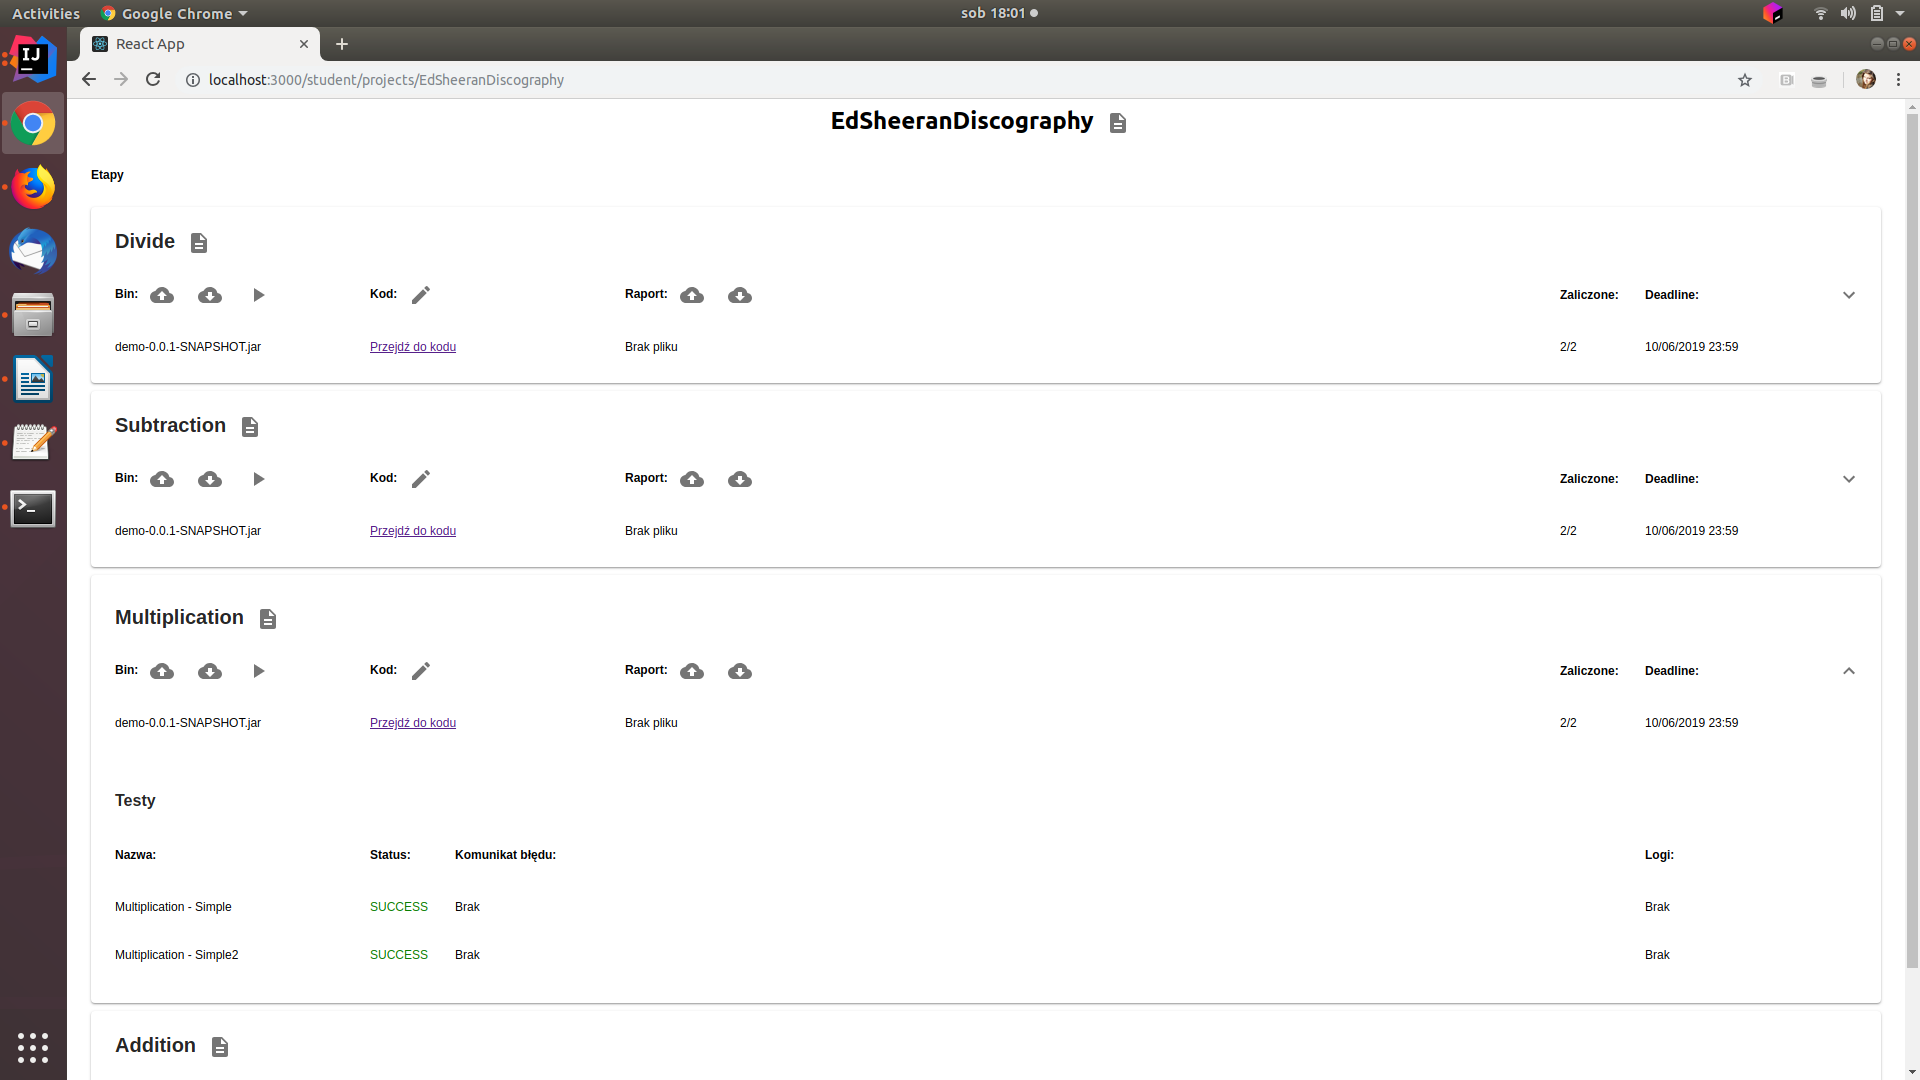
\includegraphics[width = 13cm]{chapter04/lecturer_interface_view.png}
    \caption{Interfejs prowadzącego - podgląd postępów studentów (źródło własne).}
    \label{fig:lecturer-interface-view}
\end{figure}

Prowadzący ma umożliwiony wgląd w:
\begin {itemize}
    \item Aktualną punktację projektu dla grupy.
    \item Liczbę prób podjętych przez daną grupę, dla każdego z etapów.
    \item Daty wykonania poszczególnych prób oraz ich statusy.
    \item Pełne komunikaty błędów i logi z ostatniej wykonanej przez studentów próby.
    \item Link do kodu źródłowego, który został użyty przez studentów do zbudowania programu.
    \item Sprawozdanie wykonane dla zadanego etapu.
\end {itemize}

Dodatkowo prowadzący ma możliwość edycji danych studentów z dodatkowymi uprawnieniami administratora.
Pozwalają one między innymi na edycję wprowadzonych przez studentów danych po upływie terminów realizacji poszczególnych etapów.
Są to uprawnienia, które nie powinny być nadużywane przez prowadzącego, jednak mogą okazać się użyteczne w wyjątkowych sytuacjach.


\section{Interfejs studenta}

Na rysunku \ref{fig:student-interface} został przedstawiony interfejs studenta.
Umożliwia on dodawanie i edycję danych dla kolejnych etapów projektu oraz podgląd aktualnych postępów.
W ramach projektu student ma między innymi dostęp do dwóch plików: z opisem zadania oraz definicją środowiska Dockerowego.
Interfejs umożliwia też dostęp do opisów kolejnych etapów, terminów ich realizacji i punktacji.

Dla zadanego etapu student ma możliwość załączenia:
\begin {itemize}
    \item Pliku wykonywalnego z programem, który będzie testowany na platformie.
    \item Linku do kodu, z którego został zbudowany plik wykonywalny.
    \item Sprawozdania, sporządzonego w ramach etapu.
\end {itemize}

Po załączeniu programu student ma możliwość uruchomienia go na platformie.
Wynik działania programu jest przedstawiony studentowi w postaci listy rezultatów z wykonania poszczególnych przypadków testowych.
Poszczególny rekord zawiera informacje o:
\begin {itemize}
    \item Nazwie przypadku testowego, którego dotyczy wynik.
    \item Parametrach wejściowych, które zostały użyte przy uruchomieniu programu.
    \item Statusie wykonania przypadku testowego (sukces/porażka).
    \item Komunikatu błędu, w przypadku porażki.
    \item Pliku z logami z wykonania danego przypadku testowego.
\end{itemize}

W ramach podglądu postępów student ma dostęp do:
\begin {itemize}
    \item Wyników wszystkich dotychczasowych etapów.
    \item Informacji zbiorczej o liczbie zaliczonych etapów i aktualnej punktacji.
    \item Zbiorczej informacji o postępach innych grup.
    Informacja ta jest przedstawiono jako liczba grup, które zaliczyły wskazany etap w stosunku do wszystkich grup.
\end {itemize}

Student po zakończeniu odpowiedniej liczby etapów wchodzących w skład zdefiniowanego procesu integracji ma możliwość uruchomienia tego procesu.
Wynik działania procesu jest reprezentowany w taki sam sposób jak wynik uruchomienia poszczególnego etapu.